documentclass
\documentclass[tikz,border=3mm]{standalone}
\usepackage{amsmath}
\begin{document}
\tikzset{declare function={R(\x,\y)=floor(mod(\x,5))+floor(mod(\y,5))/5;}}
\tikzset{declare function={Rmax(\x,\y)=max(R(\x,\y),floor(\y/5));}}
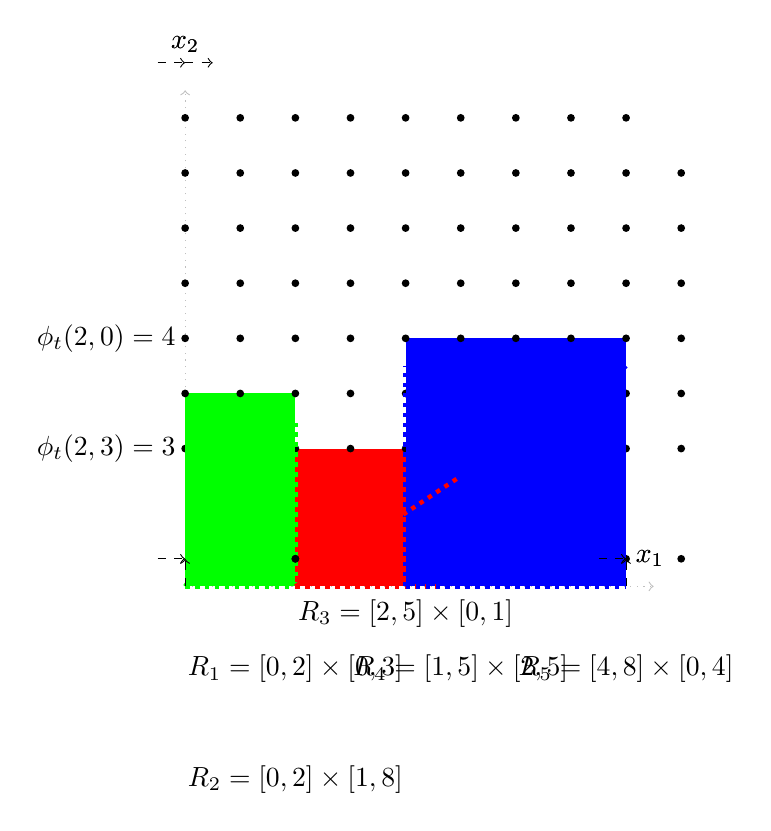
\begin{tikzpicture}[scale=0.7]
    \draw[gray!50,dotted,thin,->](0,-0.5)--+(0,9);
    \draw[gray!50,dotted,thin,->](0,-0.5)--+(8.5,0);
    \draw[ultra thick,red,fill=red,draw opacity=0] (2,0) rectangle (5,2);
    \draw[ultra thick,blue,fill=blue,draw opacity=0] (4,0) rectangle +(4,4);
    \draw[ultra thick,green,fill=green,draw opacity=0] (0,0) rectangle +(2,3);
    \node[right] at (8,0) {$x_{1}$};
    \node[above] at (0,9) {$x_{2}$};
    \foreach \i/\col [count=\j from 0] in {{(2,0)/black},{(3,0)/black},{(4,0)/black},{(5,0)/black},{(6,0)/black},{(7,0)/black},{(8,0)/black},{(9,0)/black},{(0,2)/black},{(1,2)/black},{(2,2)/black},{(3,2)/black},{(4,2)/black},{(5,2)/black},{(6,2)/black},{(7,2)/black},{(8,2)/black},{(9,2)/black},{(0,3)/black},{(1,3)/black},{(2,3)/black},{(3,3)/black},{(4,3)/black},{(5,3)/black},{(6,3)/black},{(7,3)/black},{(8,3)/black},{(9,3)/black},{(0,4)/black},{(1,4)/black},{(2,4)/black},{(3,4)/black},{(4,4)/black},{(5,4)/black},{(6,4)/black},{(7,4)/black},{(8,4)/black},{(9,4)/black},{(0,5)/black},{(1,5)/black},{(2,5)/black},{(3,5)/black},{(4,5)/black},{(5,5)/black},{(6,5)/black},{(7,5)/black},{(8,5)/black},{(9,5)/black},{(0,6)/black},{(1,6)/black},{(2,6)/black},{(3,6)/black},{(4,6)/black},{(5,6)/black},{(6,6)/black},{(7,6)/black},{(8,6)/black},{(9,6)/black},{(0,7)/black},{(1,7)/black},{(2,7)/black},{(3,7)/black},{(4,7)/black},{(5,7)/black},{(6,7)/black},{(7,7)/black},{(8,7)/black},{(9,7)/black},{(0,8)/black},{(1,8)/black},{(2,8)/black},{(3,8)/black},{(4,8)/black},{(5,8)/black},{(6,8)/black},{(7,8)/black},{(8,8)/black}}
        {\fill[color=\col] \i circle[radius=2pt];}
    \node at (4,-1){$R_3=[2,5]\times[0,1]$}; 
    \node at (2,-2){$R_1=[0,2]\times[0,3]$}; 
    \node at (2,-4){$R_2=[0,2]\times[1,8]$}; 
    \node at (5,-2){$R_4=[1,5]\times[2,5]$}; 
    \node at (8,-2){$R_5=[4,8]\times[0,4]$}; 
    \draw[ultra thick,green,fill=green,draw opacity=0] (0,-0.5) rectangle +(2,3);
    \draw[ultra thick,red,fill=red,draw opacity=0] (2,-0.5) rectangle +(3,2);
    \draw[ultra thick,blue,fill=blue,draw opacity=0] (4,-0.5) rectangle +(4,4);
    \draw[dotted,ultra thick,red] (2,-0.5)--+(0,3);
    \draw[dotted,ultra thick,blue] (4,-0.5)--+(0,4);
    \draw[dotted,ultra thick,green] (0,-0.5)--+(2,0);
    \draw[dotted,ultra thick,green] (0,-0.5)--+(2,3);
    \draw[dotted,ultra thick,green] (2,-0.5)--+(0,3);
    \draw[dotted,ultra thick,red] (2,-0.5)--+(3,0);
    \draw[dotted,ultra thick,red] (2,-0.5)--+(3,2);
    \draw[dotted,ultra thick,blue] (4,-0.5)--+(4,0);
    \draw[dotted,ultra thick,blue] (4,-0.5)--+(4,4);
    \draw[->,thin,dashed] (0,-0.5)--+(0,0.5);
    \draw[->,thin,dashed] (-0.5,0)--+(0.5,0);
    \draw[->,thin,dashed] (8,-0.5)--+(0,0.5);
    \draw[->,thin,dashed] (7.5,0)--+(0.5,0);
    \draw[->,thin,dashed] (0,9)--+(0.5,0);
    \draw[->,thin,dashed] (-0.5,9)--+(0.5,0);
    \node[right] at (8,0) {$x_{1}$};
    \node[above] at (0,9) {$x_{2}$};
    \foreach \i/\col [count=\j from 0] in {(2,0)/black}{\fill[color=\col] \i circle[radius=2pt];}
    \node[left] at (0,2){$\phi_t(2,3)=3$};
    \foreach \i/\col [count=\j from 0] in {(2,0)/black}{\fill[color=\col] \i circle[radius=2pt];}
    \node[left] at (0,4){$\phi_t(2,0)=4$};
    \node[right] at (8,0){};
\end{tikzpicture}
\end{document}